\documentclass[a4paper]{article}

\usepackage[spanish]{babel}
\usepackage[utf8]{inputenc}
\usepackage{xcolor}
\usepackage[colorlinks=true, urlcolor=black]{hyperref}
\usepackage{graphicx}

\definecolor{shadecolor}{RGB}{220,220,220}

\title{Informe sobre Apache Nutch}

\date{}

\begin{document}
\setlength{\voffset}{-1in}
\setlength{\textheight}{680px}
\setlength{\headsep}{30px}
\maketitle

\section{Motivación}

En esta asignatura hemos realizado varios A+, pequeñas exploraciones en tecnologías, nuevas para nosotros pero sencillas de comprender, de manera que nos sirvan para tener una visión más amplia de distintas herramientas. En esta ocasión hemos querido aprovechar el aprendizaje de una nueva tecnología para, si es posible, seguir trabajando sobre ella más tarde en un proyecto de investigación. 

\section{Introducción}

Apache Nutch es un crawler web, una herramienta que sirve para recorrer y extraer información de la web. Nuestro objetivo es realizar una pequeña búsqueda, extraer la información de las páginas y obtener los objetos representados sobre el html con un esquema de Microdata, de forma que podríamos enlazar estos productos desde nuestro sistema web.

\section{Instalación}

Apache Nutch se puede adquirir desde la página oficial del proyecto, mostrada en la bibliografía. También podemos encontrar numerosos tutoriales en esta página, aunque muchos están desactualizados y la documentación no es la más deseable.

Nuestro mayor problema al intentar utilizar Apache Nutch ha sido trabajar con la máquina de desarrollo que se ha dado en esta asignatura. Apache Nutch esta preparado para ejecutarse desde un sistema Linux, por lo que para ejecutarlo desde Windows necesitábamos acudir a una herramienta, cygwin, que solucionara los problemas encontrados. Pero cygwin dejo de dar soporte a Windows XP hace ya varios años, por lo que encontrar una versión de cygwin que pudiéramos instalar en la máquina virtual fue también complicado. Al conseguirlo nos encontramos con un problema más. En la versión que encontramos compatible con Windows XP, cygwin no era capaz de ejecutar los scripts de crawling de apache a no ser que lo hiciéramos siguiendo una ruta sin espacios. Como el usuario student no tiene permiso de escritura en la raíz del disco C, necesitamos cambiar al usuario boss para continuar.

Por comodidad hemos preferido trabajar finalmente desde la máquina host, que en este caso es un sistema Ubuntu donde la herramienta Apache Nutch no daba tantos problemas. Hemos usado la version 1.12 y la hemos compilado usando Apache ant.

\begin{figure}
\caption{Esquema de Nutch}
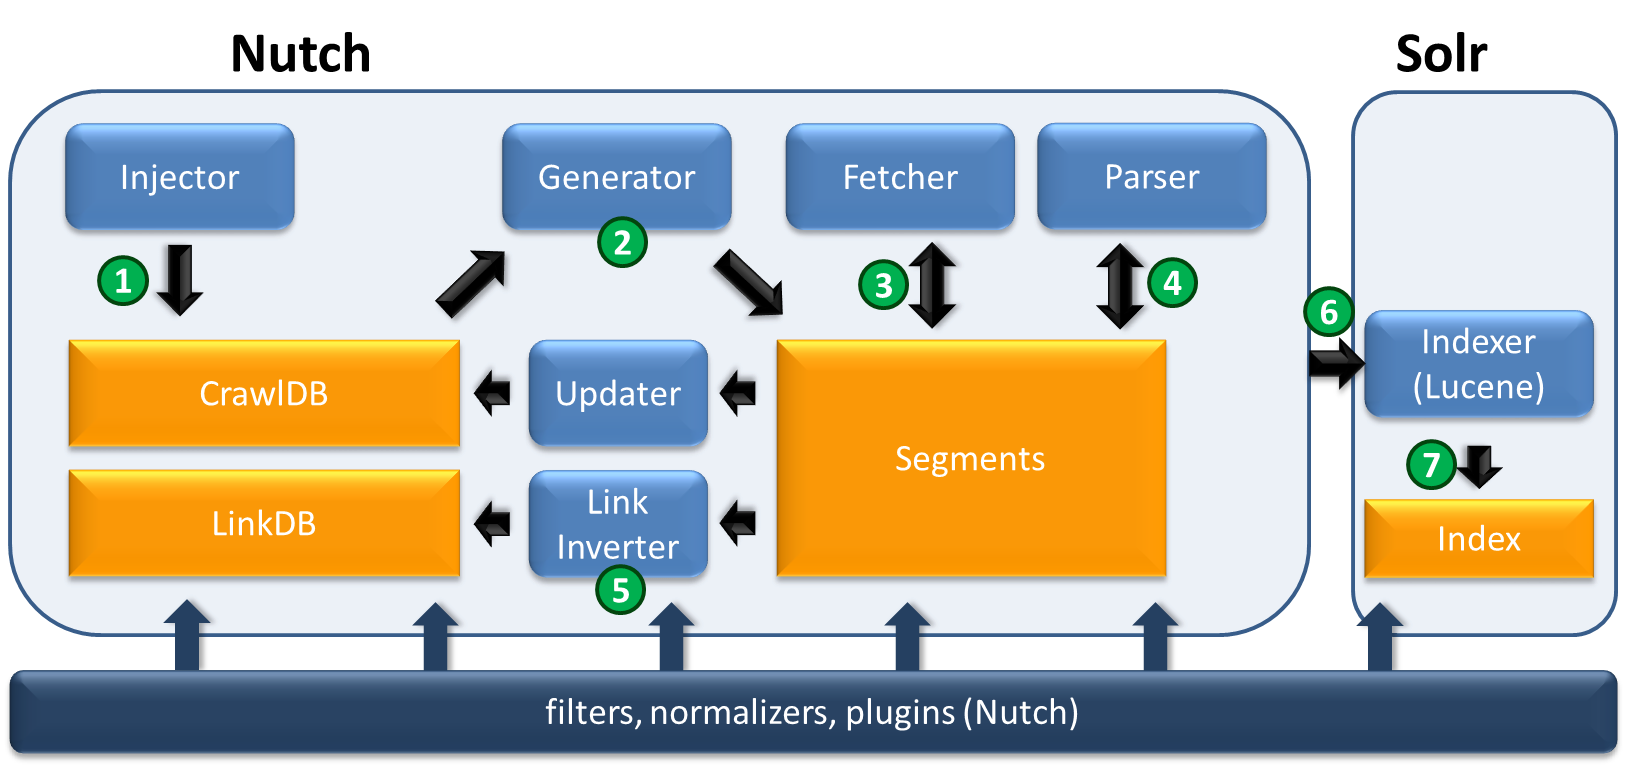
\includegraphics[width=\linewidth]{3RVif}
\label{fig:esquema}
\end{figure}

\section{Crawling}

Como hemos comentado, la documentación de nutch no es tan amplia como sería deseable, pero tras algunos usos hemos comprendido parte del proceso. Apache nutch viene con dos scripts preparados, nutch y crawl. El script crawl es más simple, y realmente lo que hace es acudir a nutch varias veces para automatizar todo el proceso de crawling siguiendo los comandos más típicos del script nutch. Usar directamente el script nutch da más libertad a un usuario avanzado de esta herramienta a la hora de hacer el crawling.

 Para utilizar el script crawl tan solo es necesario darle como entrada tres cosas: un directorio donde debe encontrarse un archivo seed.txt con los enlaces iniciales a explorar, un directorio de salida para los resultados y un número de rondas en las que iterar.  En cada iteración el algoritmo se realimenta con las nuevas URLs encontradas desde las URLs que exploro en primer lugar. Quizás lo que le falta al script crawl para que esta herramienta sea más completa es incluir en el proceso alguna extracción de los datos, ya que tras lanzar este script lo que obtendremos será un conjunto de archivos binarios organizados en tres carpetas: crawldb, linkdb y segments. Estas carpetas se corresponden con bases de datos que usa Nutch internamente, como puede verse en la figura~\ref{fig:esquema}. Dentro de la carpeta segments encontraremos una carpeta distinta para cada iteración realizada. Si volvemos a lanzar el script indicando en el directorio de salida uno que ya tiene las bases de datos de una búsqueda anterior, este no solo explorará las URLs dadas en el seed, si no también las encontradas anteriormente y almacenadas en sus bases de datos.

Una vez que tengamos los datos, lo que a nosotros nos interesa es lo que se ha guardado en la base de datos segments. Ahí esta toda la información sobre las URLs exploradas, y las que han quedado en frontera sin explorar. Para extraer la información tenemos muchas opciones disponibles en el script nutch. Por ejemplo podemos extraer todos los html de las páginas exploradas con la opción dump. Con la opción readseg podemos extraer más información, así como información más concreta. Por ejemplo, con -get se puede extraer información sobre una URL concreta, en vez de sobre todas las exploradas, y con -list podemos obtener información sobre el momento en el que empezó y acabó la búsqueda de un segmento, así como el número de URLs generadas, encontradas y exploradas. 

Con una sola URL en el archivo seed.txt, en dos o tres iteraciones el proceso puede ser lento, dependiendo de la cantidad de páginas enlazadas que tenga la original. Esto se debe a que para cada URL analizada nutch introduce un retardo, para simular el componente humano y que no se rechace la petición. Este retardo es de 5 segundos por defecto.

Podemos configurar un filtro de URLs a explorar o a ignorar en el archivo, por ejemplo, para que no salga de cierto dominio, o se salte páginas que cumplan cierto patrón. Para ello tenemos que añadir los patrones, definidos con expresiones regulares (regex) en conf/regex-URLfilter.txt.

\section{Scraping}

Una vez obtenido los distintos archivos html, nos interesa sacar de ellos la microdata. Como primera aproximación, realizamos un pequeño programa java para, dada una página concreta a la que le habíamos aplicado el crawling, nos diera la URL del producto, su nombre, su precio y su imagen. El problema de esta solución, es, por supuesto, que es completamente adaptada al caso particular. Es una solución \textit{ad hoc} que querríamos mejorar. El problema es que conseguir sacar la información, sea cual sea el esquema de Microdata utilizado, en cualquier página, no es un algo trivial. Quizás no es complicado, pero si muy trabajoso. 

Por este motivo buscamos alguna librería que hiciera esto, y encontramos apache any23. Con any23 podemos sacar de un html los ItemScope que contiene. Los modela como objetos que tienen como atributo, entre otros, un map con todos los itemProp del itemScope. Además, también permite obtener estos objetos como JSON.

\begin{figure}[h]
\caption{Lista de iteraciones}
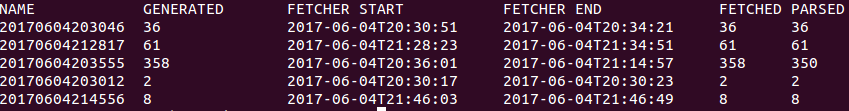
\includegraphics[width=\linewidth]{lista}
\label{fig:lista}
\end{figure}

\section{Ejemplo}

Vamos a realizar un pequeño ejemplo controlado. Hemos elegido la web http://www.wanyma.com/ porque tiene sus productos esquematizados con Microdata. Vamos a hacer un crawling de todos los piensos que tengan para perros. Para ello hemos puesto como seed la página http://www.wanyma.com/perro\slash pienso/, y como filtro regex hemos incluido la linea +\^{}http://www.wanyma.com\slash perro/pienso/ y hemos quitado la linea +., de forma que solo analizará las páginas dentro de la categoría pienso para perros de la página. Realizamos un crawling de seis iteraciones con la intención de recorrer todo lo que cumpla ese filtro y usamos la opción dump para extraer todos los html de las páginas. Podemos ver con la opción readseg -list cuantas páginas se han tratado en cada iteración. Hemos usado los comandos:

\$./bin/crawl urls piensoCrawl 6

\$./bin/nutch dump -segment piensoCrawl/segments -outputDir piensoCrawl\slash dump/

\$./bin/nutch readseg -list -dir piensoCrawl/segments


Como vemos en la figura~\ref{fig:lista} solo han hecho falta 5 iteraciones para completar la búsqueda. Ahora que ya tenemos la información, podemos utilizar any23 para extraer los esquemas Microdata. Hemos hecho un pequeño ejemplo en el que simplemente filtramos los que son de tipo Product y los hemos contado, dando un total de 402 productos.

\section{Consideraciones}
Podríamos haber ampliado el proyecto introduciendo el esquema producto en la base de datos mysql de Acme-Pet y volcando los ItemScope de este esquema en nuestra base de datos, y así poder mostrarla fácilmente en nuestra aplicación, pero el tiempo a jugado en nuestra contra y hemos preferido centrarnos en ampliar conocimientos sobre la tecnología que estábamos usando.

Adjuntamos con este documento un proyecto java que tiene dos aplicaciones, ExtractData y NutchMicrodataParser. La primera es la aproximación ad hoc que comentamos anteriormente, que funciona con dos productos ejemplos (los html los hemos extraído con una crawling de una iteración sobre la página del producto directamente). La segunda es la aplicación donde implementamos la librería any23 y que usamos en el ejemplo anterior.

\section{Bibliografía}

\url{http://nutch.apache.org/}

\url{https://any23.apache.org/}


\end{document}